\chapter{Studium problematiky}
\label{studium}
Tato kapitola se zabývá stručným popisem problematiky. Obsahuje informace potřebné k~pochopení tématu, správnému návrhu a implementaci aplikace. Je zde vysvětlen pojem genealogie, způsob jakým jsou ukládány informace v~matričních knihách a popsán formát vstupních souborů aplikace.
\section{Genealogie}
Genealogie\footnote{Genealogie - pochází z~řeckých slov genea = původ a logos = znalost} je odvětví zabývající se rodovými vztahy mezi jedinci určitého druhu. Zkoumá tedy rodové souvislosti. Zabývá se buď studiem jednotlivých osobností, nebo sledováním proměn jednotlivých druhů vztahů.

Genealogii považujeme za jednu z~metod genetického výzkumu. Základem genealogické metody je grafické zaznamenání rodových vztahů mezi jedinci v~jednotlivých generacích. Tuto grafickou podobu nazýváme rodokmen~\cite{genealogie}. 

\subsection{Genealogické diagramy}
Jedná se o~schéma reprezentující vztahy v~rámci rodiny pomocí stromové struktury. V~následujících podkapitolách budou popsány nejznámější schémata. K~popisu diagramů bylo v~této podkapitole čerpáno z~webové stránky Václava Příborského~\cite{geneDiagramy}.
\subsubsection{Rodokmen}
Jedná se o~základní a nejjednodušší schéma. Začíná u~zakladatele rodu, tedy nejstaršího známého předka. Zahrnuje jeho děti a potomky všech jejich synů, kteří si založili vlastní rodinu. Zkoumáme pouze potomky synů, jelikož syn je obvykle nositelem příjmení, kdežto dcera nikoliv. Příjmení je totiž typickým znakem rodokmenu. Pomocí rodokmenu lze zkoumat mohutnost celého rodu, počty manželství v~jednotlivých generacích a mnoho dalších zajímavých informací. Schéma rodokmenu se nachází na obrázku~\ref{figure_rodokmen}.

\begin{figure}[H]
	\centering
	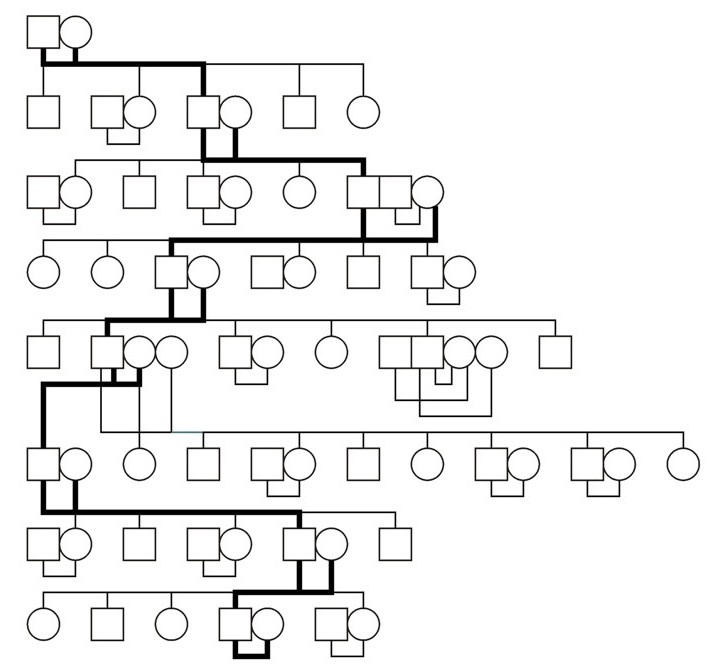
\includegraphics[width=80mm]{obrazky-figures/rodokmen.jpg}
	\caption[Schéma rodokmenu]{Schéma rodokmenu [převzato ze stránky \cite{schema}]}
	\label{figure_rodokmen}
\end{figure}

\subsubsection{Rozrod}
Rozrod oproti rodokmenu zahrnuje všechny potomky zakladatele rodu. Je tedy rozšířen i o~potomky dcer. Dají se z~něj vysledovat osudy celé široké rodiny. V~genealogii se jedná o~nejrozsáhlejší a nejsložitější schéma. Obsahuje větší počet osob než rodokmen, je tak i náročnější na vytvoření, ale jsme z~něj schopni získat více informací a sledovat veškeré potomstvo. Schéma rozrodu se nachází na obrázku~\ref{figure_rozrod}.

\begin{figure}[H]
	\centering
	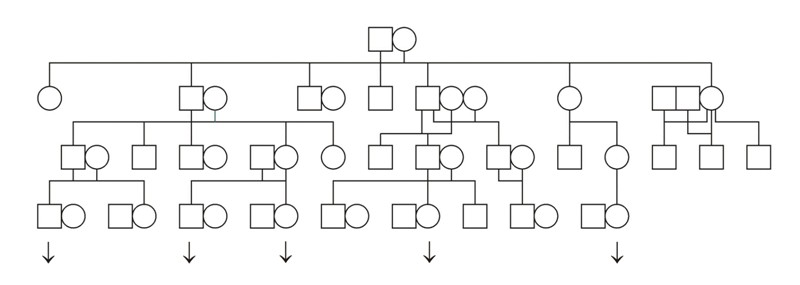
\includegraphics[width=95mm]{obrazky-figures/rozrod.jpg}
	\caption[Schéma rozrodu]{Schéma rozrodu [převzato ze stránky \cite{schema}]}
	\label{figure_rozrod}
\end{figure}

\subsubsection{Vývod}
Vývod vychází od zkoumané osoby směrem nahoru. Zahrnuje tedy mužské i ženské předky dané osoby směrem do minulosti. Vypovídá o~generacích rodičů a prarodičů výchozí osoby. Lze z~něj získat větší znalost o~rodinných kořenech osoby a zkoumat předchozí generace. Vývod můžeme rozdělit na agnátní a kognátní. Agnátní sleduje pouze mužskou linii, kognátní ženskou. Schéma vývodu se nachází na obrázku~\ref{figure_vyvod}.

\begin{figure}[H]
	\centering
	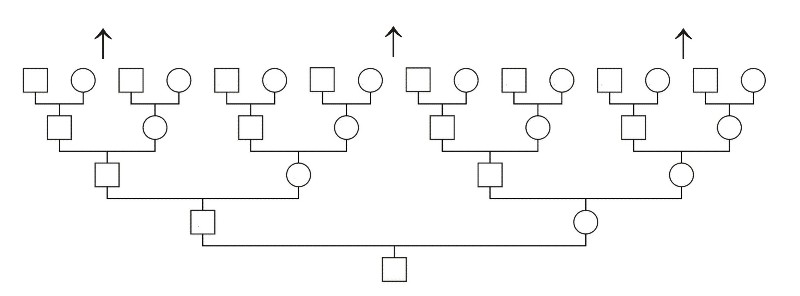
\includegraphics[width=95mm]{obrazky-figures/vyvod.jpg}
	\caption[Schéma vývodu]{Schéma vývodu [převzato ze stránky \cite{schema}]}
	\label{figure_vyvod}
\end{figure}

%\subsection{Jak provést genealogický výzkum}
\section{Matriky}
Matriky jsou základním pramenem dat při provádění genealogického výzkumu. Jedná se o~knihy vedené ve stylu úředního seznamu jmen. Obsahují různé informace související s~danou událostí a osobou. Matriky jsou tedy seznamem uchovávajícím záznamy o~narození, sňatcích a úmrtí dané osoby. Tyto seznamy jsou vedeny matrikáři na patřičných matričních úřadech. Takovým úřadem může být například obecní úřad, úřad městské části nebo městského obvodu.

Matriky rozdělujeme na dva druhy podle jejich dostupnosti, na živé a mrtvé. Živé matriky jsou takové, které v~sobě obsahují záznamy u~nichž neuplynulo od posledního narození 100 let, a nebo 75 let od posledního sňatku či úmrtí. Takové matriky nejsou veřejně přístupné a smí se do nich nahlížet pouze za přítomnosti matrikáře a při splnění alespoň jedné z~určitých podmínek, které jsou popsány na webu ministerstva vnitra České republiky\footnote{\url{https://www.mvcr.cz/migrace/docDetail.aspx?docid=21814471}}. Ostatní matriky prohlašujeme za mrtvé a jsou veřejně dostupné na úřadech či v~digitální podobě.

Z~počátku se všechny druhy záznamů zapisovaly do jedné knihy společně. Později, zhruba od druhé poloviny 18. století, se začaly záznamy pro jednotlivé události zapisovat do pro ně konkrétních matrik. Typy těchto matrik jsou popsány v~následujících podkapitolách~\cite{Matriky}.

\subsection{Matriky narození}
V~této knize nalezneme údaje týkající se narození dané osoby. Můžeme zde nalézt jméno i příjmení, datum narození ale i křtu, pohlaví nebo třeba náboženství. V~těchto knihách ovšem často nalezneme také údaje nejen o~této osobě, ale také jméno, stav a rod jeho matky, otce, křtitele nebo i kmotra. Jak vypadá záznam v~takové matrice je ukázáno na obrázku~\ref{figure_birth_parishbook}.

\subsection{Matriky úmrtí}
Úmrtní matriky obsahují kromě základních informací jako je jméno, datum a číslo domu, také informace specifické k~této události. Tedy stáří zemřelého a příčinu úmrtí.

\subsection{Matriky oddání}
Tyto matriky v~sobě uchovávají záznamy o~oddání dvou osob. Obsahují základní informace o~události, tedy datum sňatku, číslo popisné domu, a dále pak informace o~osobách účastnících se sňatku. Zde se opět řadí základní informace jako jsou jména, náboženství, stáří, ale také třeba stav osoby (svobodný/vdovec). Můžeme zde nalézt i údaje o~svědcích.

\begin{figure}[H]
	\centering
	\includegraphics[width=125mm]{obrazky-figures/Matricni\_zaznam\_narozeni.PNG}
	\caption[Matriční záznam]{Část snímku č. 111 z~matriky narození [převzato z~archivu \cite{snimek}]}
	\label{figure_birth_parishbook}
\end{figure}

\subsection{Digitalizace}
V~roce 2007 započala digitalizace matrik v~rámci České republiky. Byla iniciována americkou genealogickou společností Family Search\footnote{Family Search - \url{https://www.familysearch.org/en/}}. Digitalizace matrik umožňuje komukoliv nahlédnout do knihy bez nutnosti cestovat do archivu, kde jsou matriky uloženy. Digitalizované knihy se nacházejí na celkově osmi online archivech\footnote{Rozcestník - \url{https://digi.ceskearchivy.cz/Matriky-Matricni-rozcestnik-Ceske-republiky}}, rozdělení je znázorněno na obrázku~\ref{figure_archives_map}. Tyto weby umožňují vyhledávat knihy na základě parametrů. Nejedná se o~přepis matrik do digitální podoby, ale o~ofocení jednotlivých stránek matriční knihy a zveřejnění těchto fotek~\cite{digitalizaceMatrik}.

\begin{figure}[H]
	\centering
	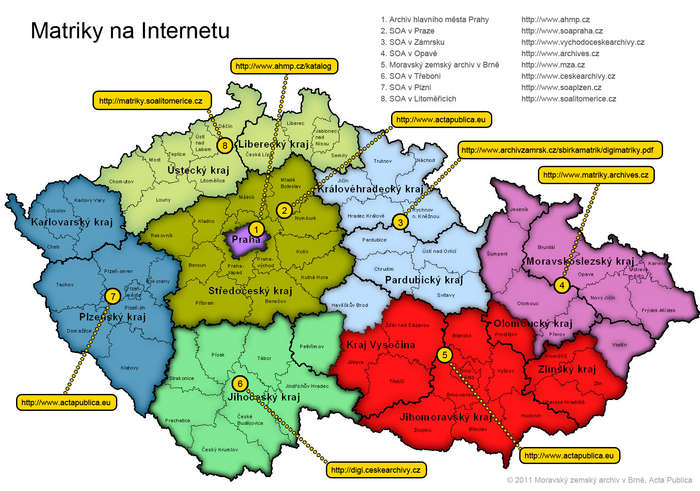
\includegraphics[width=130mm]{obrazky-figures/mapa.jpg}
	\caption[Rozdělení archivů]{Rozdělení archivů ČR [převzato ze stránky \cite{mapa}]}
	\label{figure_archives_map}
\end{figure}

\section{GEDCOM}
GEDCOM, Genealogical Data Communication, je čistě textový souborový formát určený pro ukládání a distribuci genealogických dat. Jedná se o~nejpoužívanější datový formát v~oboru genealogie. Specifikace byla vytvořena Církví Ježíše Krista Svatých posledních dnů, jež jej zpravuje dodnes. Aktuálně používaný a nejrozšířenější standart je 5.5.1, ale posledním vydaným je 7.0, jenž se snaží o~vylepšení. Implementovaná aplikace pracuje výhradně se standardem 5.5.1.

\subsection{Popis formátu}
Specifikace GEDCOM má velmi rozsáhlou dokumentaci~\cite{GEDCOM}. V~následující části z~ní budou vybrány pravidla důležité pro tuto práci.

Soubory GEDCOM končí příponou .ged. Soubor se skládá z~hlavičky, která popisuje obecné informace o~souboru (verze, kódování, aj.), množiny záznamů a speciálního ukončovacího záznamu TRLR, jenž oznamuje konec souboru.

Záznamy jsou v~souboru organizovány do hierarchické struktury po řádcích. Každý řádek záznamu je označen číselnou úrovní, indikující hloubku zanoření, kdy první řádek má hodnotu 0. Další řádky mají hodnotu vyšší a platí, že řádek s~hodnotou n+1 spadá pod řádek s~hodnotou n. Řádek s~hodnotou 0 tedy znamená začátek nového záznamu. Za úrovní může následovat křížový odkaz, který jednoznačně identifikuje danou osobu/rodinu. Odkaz je následován značkou, neboli tagem. Tag oznamuje jaká informace bude následovat. Tagů je velké množství, význam jednotlivých tagů je vysvětlen v~dokumentaci specifikace. V~tagu může být také obsažen identifikátor rodiny, do které daná osoba patří.

\subsubsection{Záznam}
Jak už bylo v~předchozím odstavci naznačeno, kromě speciálního záznamu TRLR existují dva typy záznamů. 

Prvním je záznam o~individuální osobě (INDI), jenž uchovává základní genealogické informace o~dané osobě. Nás zajímá jméno osoby a události narození (BIRT) a úmrtí (DEAT). U~každé takové události je uvedeno datum (DATE) a lokace (PLAC), kdy a kde událost proběhla. Dále tento záznam obsahuje odkazy na rodiny, kterých je osoba součástí. 

Druhým typem je záznam o~rodině (FAM). V~tomto záznamu může být popsána událost oddání (MARR). Ta je opět popsána datem a lokací. Dále tento záznam obsahuje odkazy na členy rodiny. V~rodině může mít osoba určitou roli, manžel (HUSB), manželka (WIFE), dítě (CHIL). Tento záznam může obsahovat také různé statistické hodnoty, jako například počet dětí.


\subsubsection{Datum}
Den, měsíc a rok mají přesně daný formát zápisu. Den a rok se zapisují pomocí číselné hodnoty ve tvaru DD pro den, a YYYY pro rok. Měsíc se skládá ze tří prvních písmen z~jeho anglického jména ve tvaru MMM. Datum je pak možné zapsat jako celek, tedy DD MMM YYYY, nebo postupně odebírat prvky zleva až po rok (MMM YYYY, YYYY). 

Datum může také obsahovat různé fráze, jako např.: BEF, AFT, FROM. Tyto fráze pak mohou specifikovat rozsah nebo období.

\subsubsection{Lokace}
Jediné pravidlo popisující lokaci je pravidlo hierarchie územních celků. To říká, že při zápisu lokace se mají řadit od nejmenšího po největší zleva doprava a mají být odděleny čárkami. Jinak je možné do lokace zapsat prakticky cokoliv, což všeobecně vytváří problémy při implementaci aplikací pracujících s~GEDCOM formátem.
